\begin{figure}[H]
    \subfloat[MODIS external]{\includegraphics[scale=0.45]{figs/MODIS-external.png}}
    \quad
    \subfloat[MODIS subsystems]{\includegraphics[scale=0.5]{figs/modis-sub.png}}
    \caption{MODIS (credits: wikipedia.org)}
\end{figure}
\paragraph{Introduction}
MODIS (or Moderate Resolution Imaging Spectroradiometers) is an instrument onboard the Terra(EOS AM)
and Aqua(EOS PM) satellites. Terra's orbit around the Earth is timed so that it passes from north to south
across the equator in the morning, while Aqua passes south to north over the equator in the afternoon. MODIS
is designed to provide measurements in large-scale global dynamics, including oceans, land, and cloud cover.
The Scan Mirror Assembly uses a continuously rotating double-sided scan mirror to scan $\pm55$-degrees and is
driven by a motor encoder built to operate at 100 percent duty cycle throughout the 6-year instrument design
life

\begin{figure}
    \centering
    \includegraphics[scale=0.25]{figs/aqua_orbit.png}
    \includegraphics[scale=0.25]{figs/aqua_orbit2.png}
    \caption{AQUA-MODIS orbit, credits:NASA GSFC}
\end{figure}

\paragraph{Specification}
It captures 36 spectral bands ranging in wavelength from $0.4\mu m$ to $14.4\mu m$ and at varying spatial resolutions.
Together the instruments image the entire Earth every 1 to 2 days.
It has a sun-synchronous, near-polar orbit of 705km with a swath of 2300km cross-track by
10km along the track at nadir. It has a scan rate of 20.3rpm cross track.
MODIS's temporal resolution is 1-2 days and was launched and designed to work for at least 6-years.


\paragraph{Data processing}
    \subsubsection{Sea Surface Temperature (SST)} The Sea surface temperature is observed at $11\mu m$ and $4\mu m$ for day and night respectively with $4km$ and $9km$ spatial resolution.
    In this analysis, we have utilized the $11\mu$ with $4km$ resolution daily data.

    \begin{figure}[H]
        \centering
        \includegraphics[width=\textwidth]{figs/sst_20180101.png}
        \caption{Sea Surface Temperature($^\circ C$; $11\mu$) 2018/01/01}
        {\footnotesize Processed and plotted in python with using `nctoolkit`;}
        {\footnotesize the white portions represent land mass, swaths and cloud cover.}
    \end{figure}

    \begin{figure}[H]
        \centering
        \includegraphics[width=14cm, trim={{0cm} {0.5cm} {0cm} {0cm}}, clip]{figs/sst_in_AQUA_MODIS_20180102.png}
        \caption{Sea Surface Temperature($^\circ C$; $11\mu$) 2018/01/02}
        {\footnotesize Processed and plotted using NASA Panoply with interpolations enabled}
    \end{figure}

    \paragraph{Monthly averaged}
        The daily fluctuations vanishes when we average for a month; the remaining fluctuations are called monthly temperature anamolies.

        \begin{figure}[H]
            \centering
            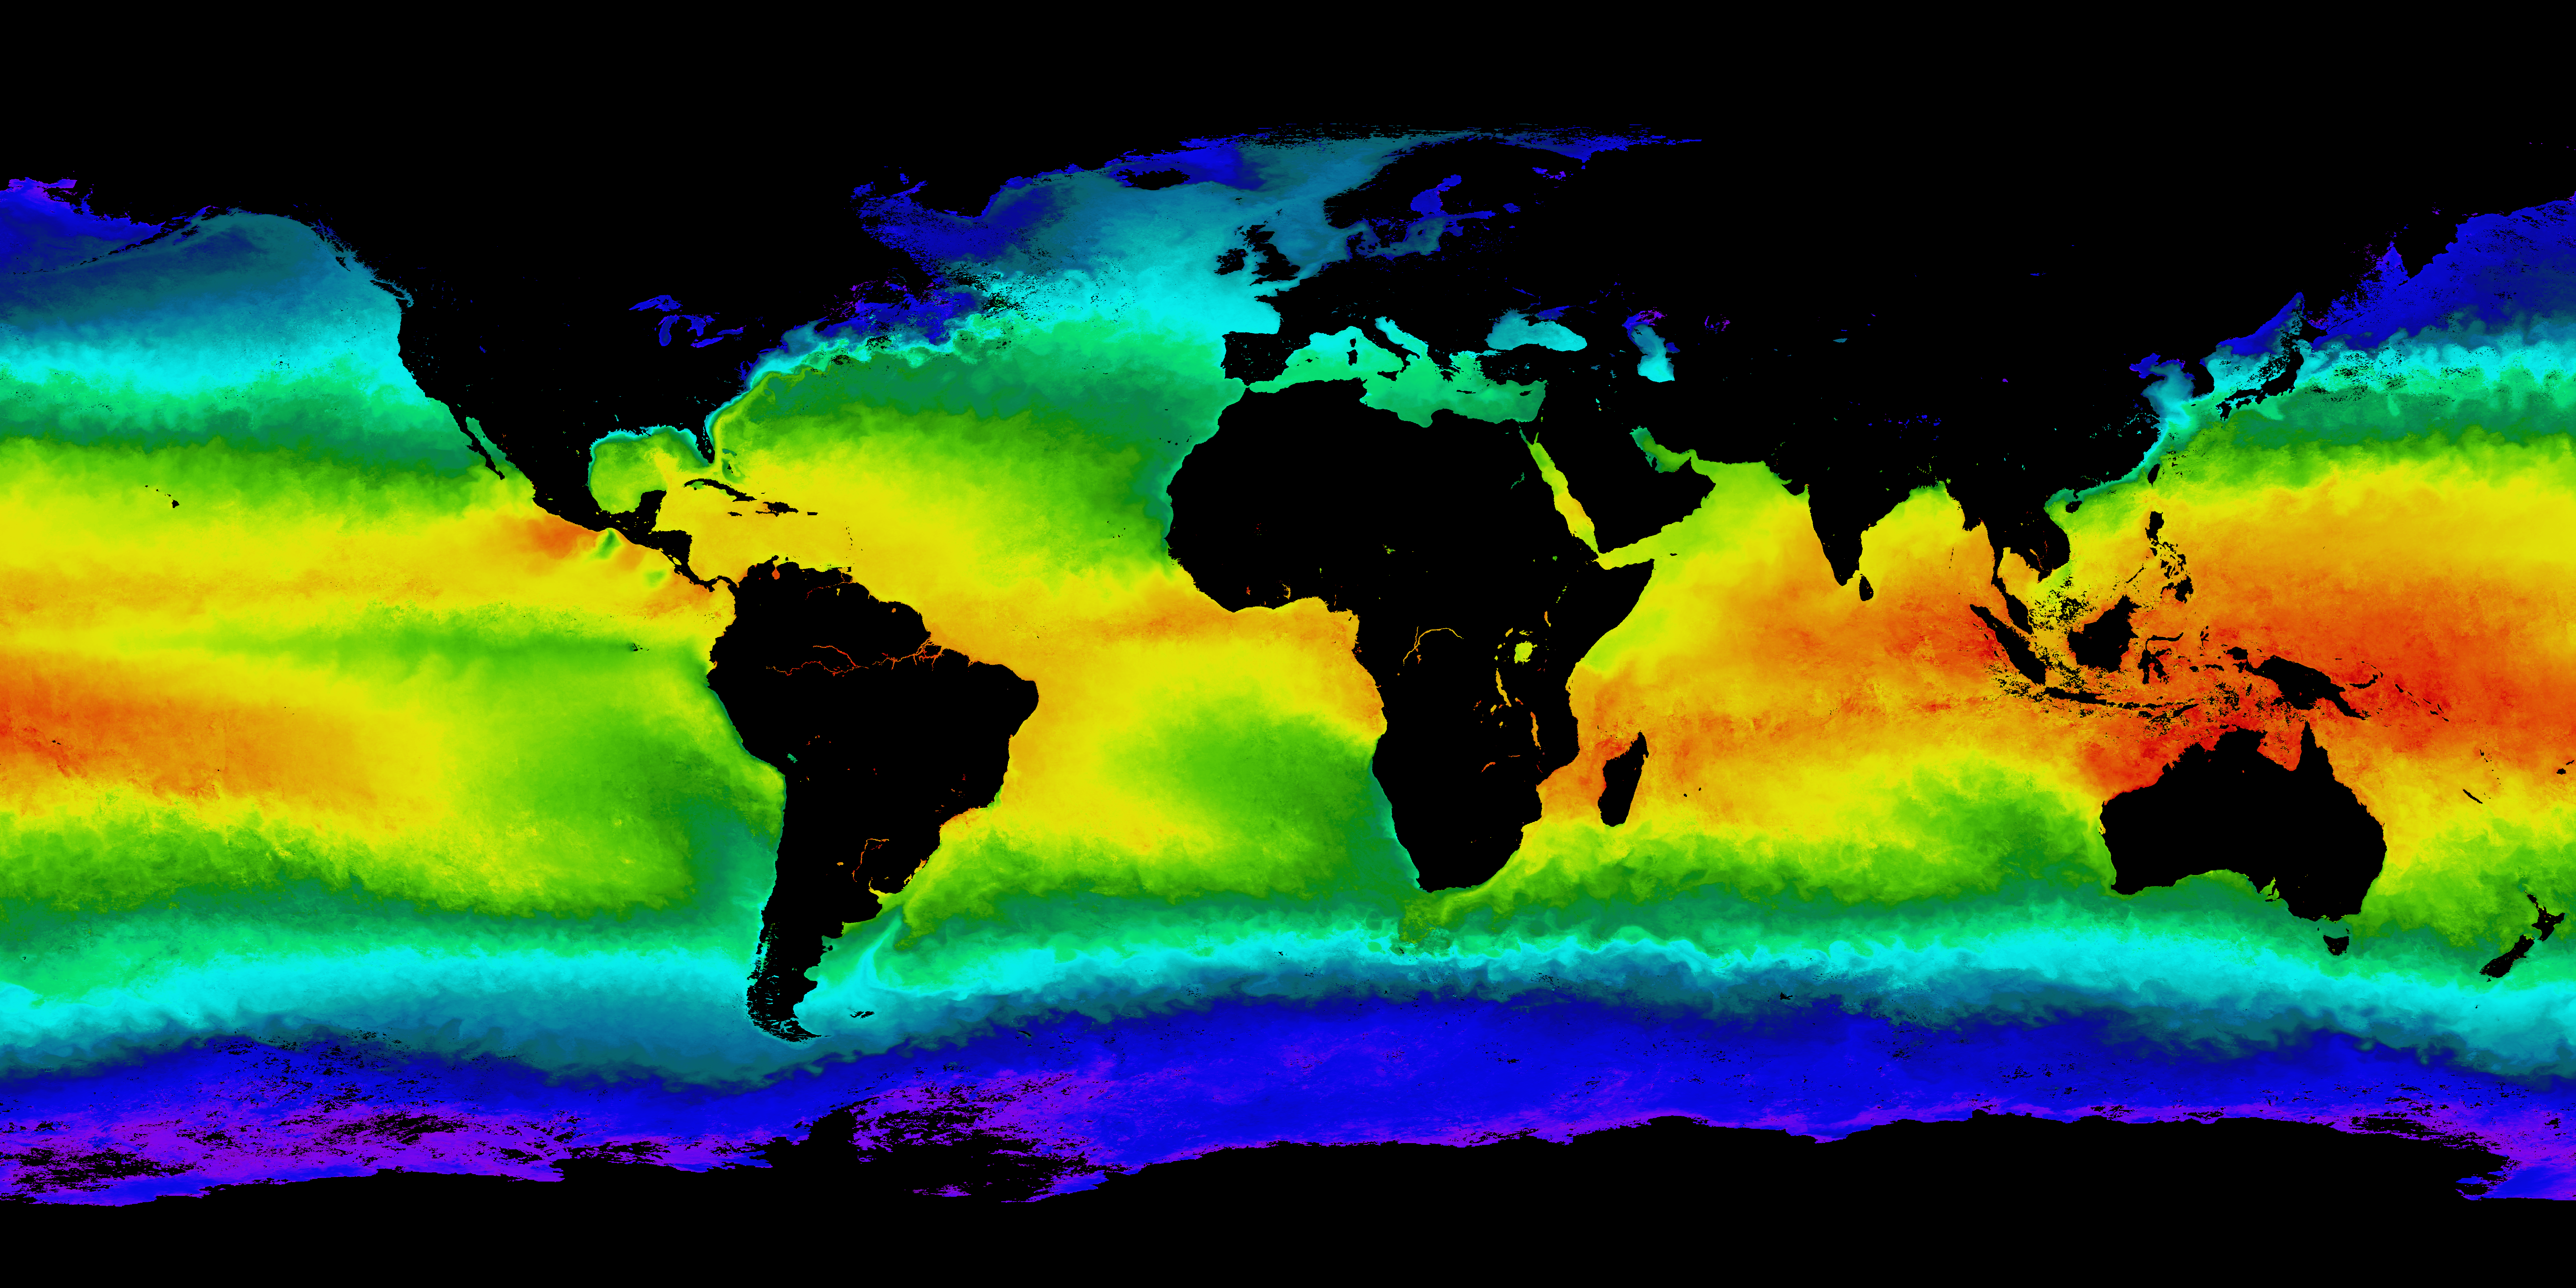
\includegraphics[width=\textwidth]{figs/AQUA_MODIS_20180101_20180131.png}
            \includegraphics[scale=0.4]{figs/sst_colorbar.png}
            \caption{Montly averged temperatures for January 2018}
        \end{figure}
    
    \subsubsection{Chlorophyll} The chlorophyll content cannot be directly measured using remote methods, so in this analysis the chlorophyll-A is computed using the NASA OCI algorithm.

    This algorithm returns the near-surface concentration of Chlorophyll-A(chlor\_a) in $mg\; m^{-3}$, calculated using an empirical relationship derived from in-situ measurements of chlor\_a and remote sensing reflectances ($R_{rs}$) in the blue-to-green region of the visible spectrum.

    In this analysis, we have utilized the $4km$ spatial resolution daily dataset.

    \begin{figure}[H]
        \centering
        \includegraphics[width=14cm, trim={{0cm} {0.5cm} {0cm} {0cm}}, clip]{figs/chlor_a_in_A2018004.png}
        \caption{Chlorophyll-A 2018/01/04}
        {\footnotesize Processed and plotted using NASA Panoply with interpolations enabled}
    \end{figure}
    
    \begin{figure}[H]
        \centering
        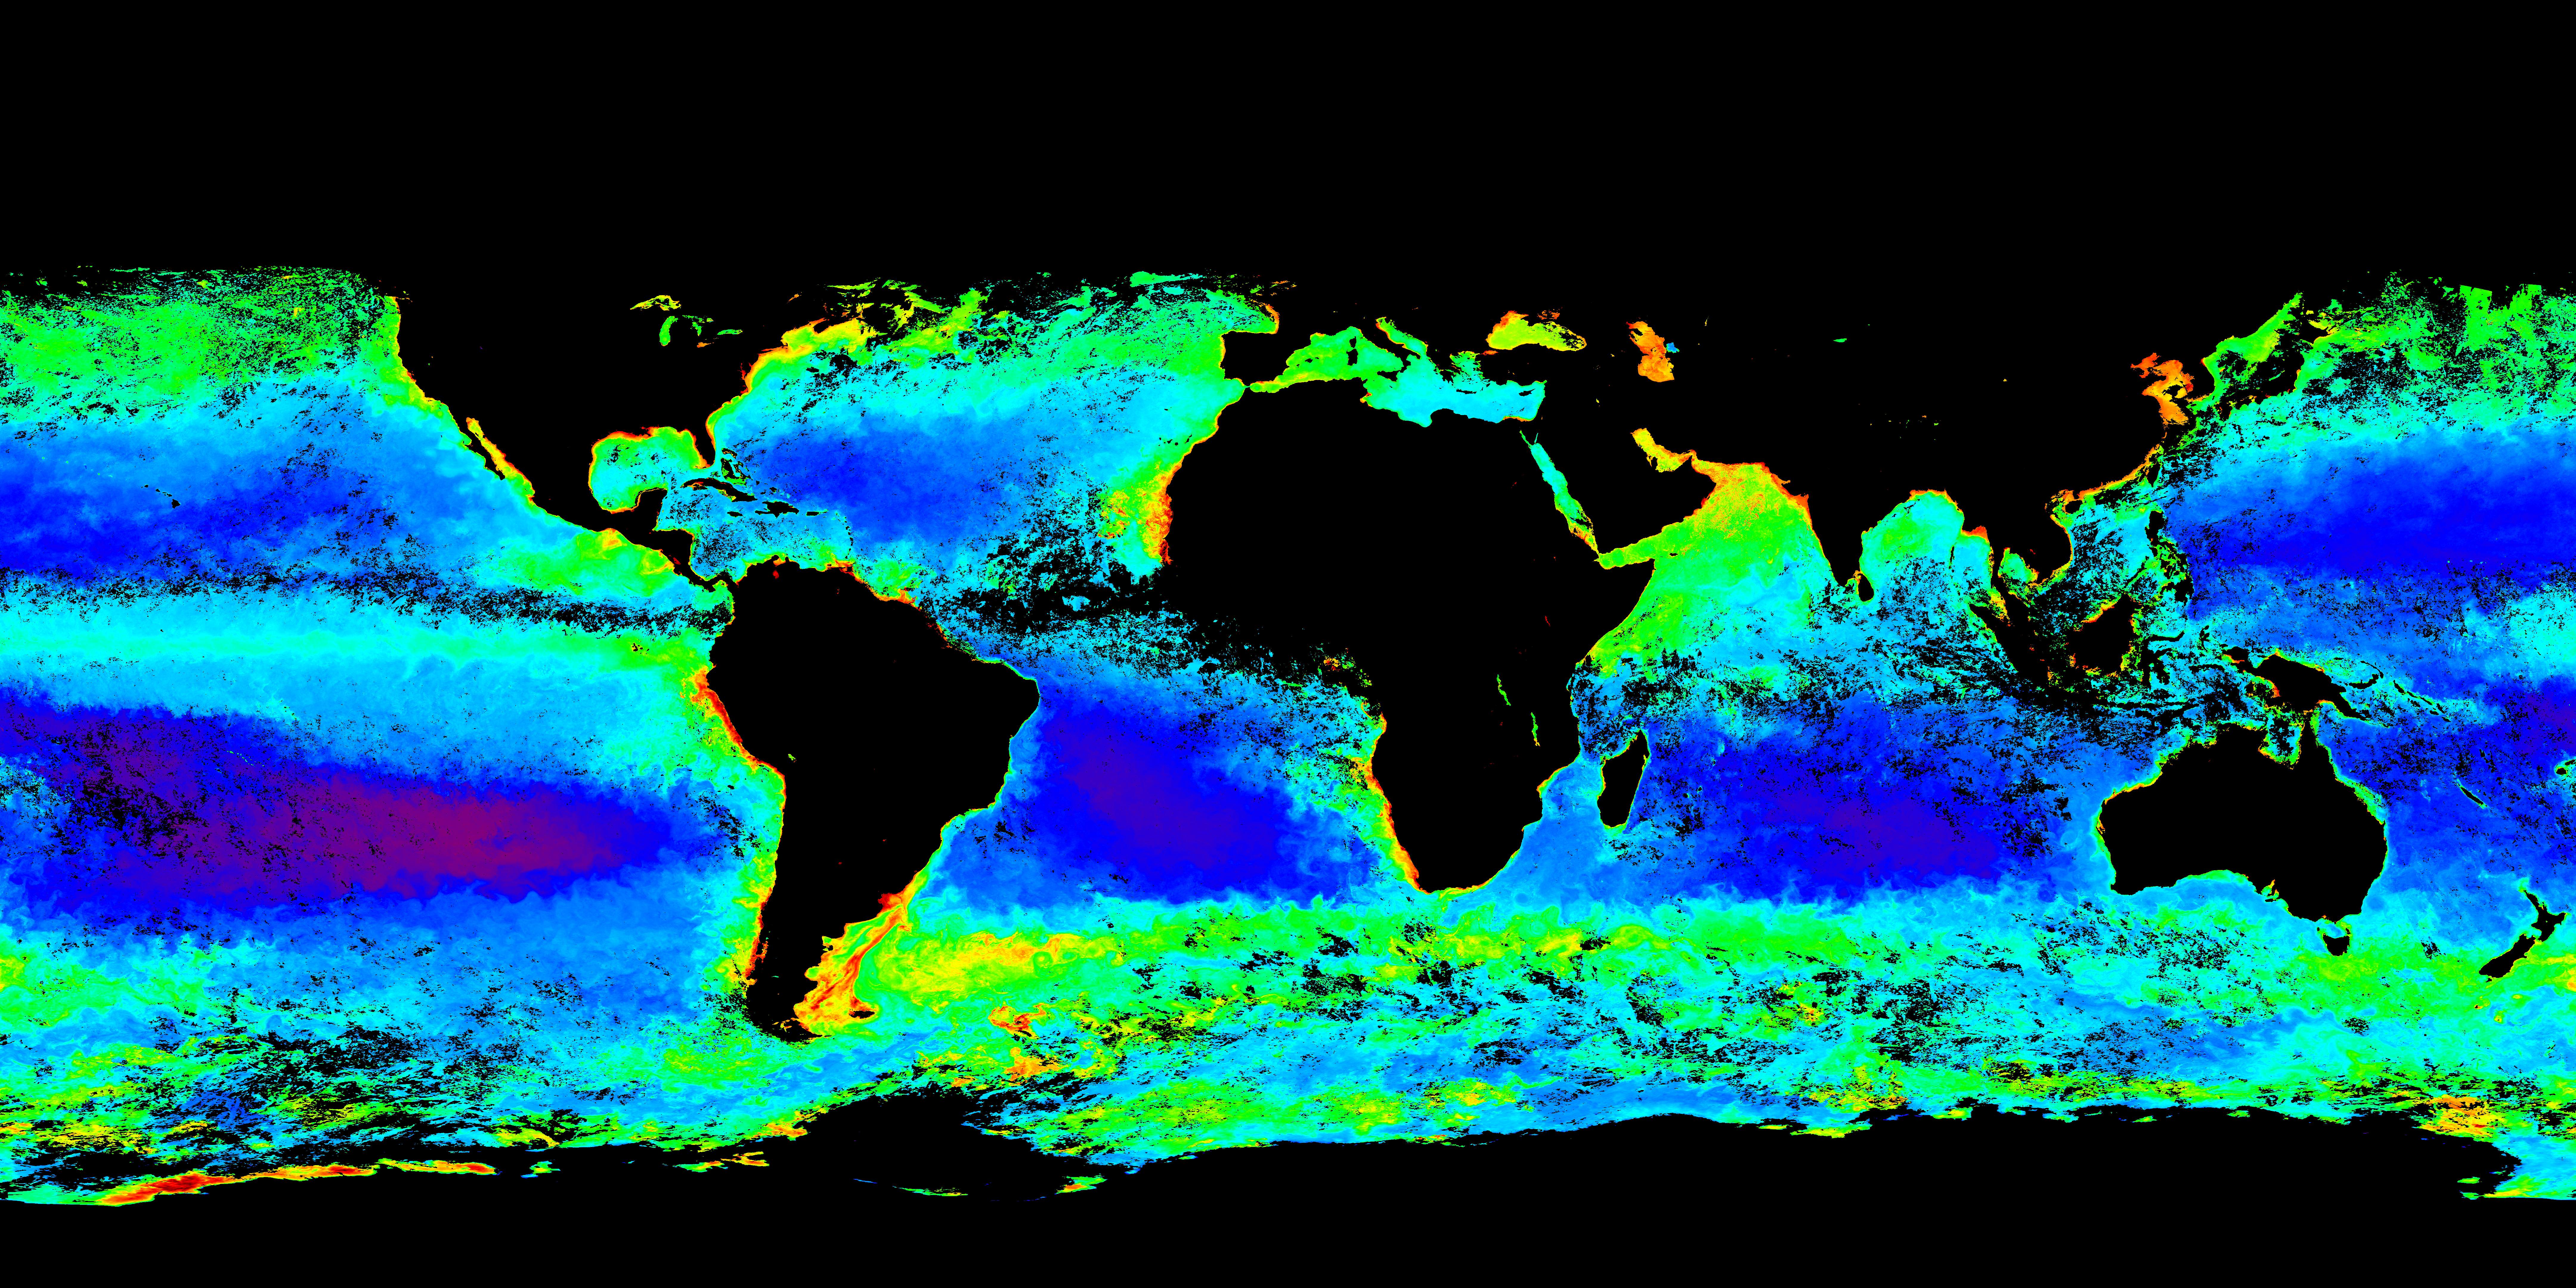
\includegraphics[width=14cm]{figs/A20180012018031png.png}
        \includegraphics[scale=0.4]{figs/chl_colorbar.png}
        \caption{Montly averged chlorophyll-a (OCI) for January 2018}
    \end{figure}

% \begin{table}[H]
%     \centering
%     \begin{tabular}{l|c|c|c}
%         \toprule\toprule
%         Band & wavelength(nm) & Spatial resolution(m) & Spectral width(nm) \\
%         \midrule
%         Band 1 - Red & $620-670$ & $250$ & $2.0$ \\
%         Band 2 - NIR & $841-876$ & $250$ & $6.0$ \\
%         Band 3 - Blue/Green & $459-479$ & $500$ & $6.0$ \\
%         Band 4 - Green & $545-565$ & $500$ & $3.0$ \\
%         Band 5 - NIR & $1230-1250$ & $500$ & $8.0$ \\
%         Band 5 - mid IR & $1628-1652$ & $500$ & $18.0$ \\ 
%         Band 5 - mid IR & $2105-2155$ & $500$ & $18.0$ \\
%         \bottomrule
%     \end{tabular}
% \end{table}